%----------------------------------------------------------------------------------------
%	PAKET-/ UND ANDERE DOKUMENT-IMPORTS
%----------------------------------------------------------------------------------------
\documentclass{scrartcl}   % Formateinstellungen
\usepackage[ngerman]{babel} % deutsche Silbentrennung
\usepackage[utf8]{inputenc} % deutsche Umlaute
\usepackage{placeins}   % verbessert Anzeige eines Floats hinter dem Befehl \FloatBarrier
\usepackage{amsfonts}   % neue Schriftanpassungen (wird von amssymb (s.u.) geladen)
\usepackage{amssymb}    % erweitert Benutzung von amsfonts (s.o.)
\usepackage{amsmath}    % Vielzahl von neuen mathematischen Umgebungen und Befehlen (wird von mathtools (s.u.) geladen)
\usepackage{mathtools}  % Verbesserung von amsmath (s.o.)
\usepackage{booktabs}   % Tabellen ohne vertikale Striche
\usepackage{siunitx}    % Einheitensystem
\usepackage[margin={0.3cm,0.3cm},font=singlespacing,labelfont=bf,labelsep=endash]{caption} % Bildunterschriften
\usepackage{wrapfig}    % Bild von Text umfließen lassen
\usepackage{sidecap}    % ermöglicht Überschriften neben Bildern / Tabellen
\usepackage{setspace}   % zum Definieren des Zeilenabstandes
\usepackage{eurosym}    % ergänzt optimales Euro-Zeichen
\usepackage[perpage,marginal]{footmisc} % ermöglicht Fußnoten und das Verändern dieser
\usepackage{graphicx}   % ermöglicht besseres Einbinden von Grafiken
\usepackage{fancyhdr}   % zum Erstellen von Kopf- und Fußzeilen
\usepackage{listings}   % ermöglicht Quellcodelisting
\usepackage{color}  % Farb-Management von Vorder- und Hintergrundfarben
\usepackage{pdfpages}   % ermöglicht das Einbinden von ganzen oder nur Teilen von PDFs
\usepackage{lineno} % Zeilenzählung
\usepackage{framed} % ermöglicht das Einrahmen von Elementen
\usepackage{pifont} % fügt Symbol-Schriften hinzu
\usepackage[hidelinks]{hyperref}    % ermöglicht das Hinzufügen von Links und Verweisen innerhalb
                                    % des PDF Dokuments und weitere Einstellungen
\usepackage[left=2.5cm,right=2cm,top=2cm,bottom=2cm,includeheadfoot]{geometry}  % Größenanpassung der Seite
%----------------------------------------------------------------------------------------


%----------------------------------------------------------------------------------------
%   KONFIGURATIONEN
%----------------------------------------------------------------------------------------
\begin{document}
\setlength{\parskip}{1ex}   % Abstand zwischen Absätzen 
\parindent 0pt  % legt Einrücke der ersten Zeile fest
\renewcommand{\thefigure}{\arabic{figure}.\alph{ab}}    % Umdefinieren von Bildnummern

\definecolor{darkblue}{rgb}{0,0,.6} % Festlegen der Farben
\definecolor{darkred}{rgb}{.6,0,0}  % Festlegen der Farben
\definecolor{darkgreen}{rgb}{0,.6,0}    % Festlegen der Farben
\definecolor{red}{rgb}{.98,0,0} % Festlegen der Farben

\lstloadlanguages{Java} % lädt Programmiersprachen
\lstset{language=Java,basicstyle=\footnotesize\ttfamily,commentstyle=\itshape\color{darkgreen},keywordstyle=\bfseries\color{darkblue},stringstyle=\color{darkred},tabsize=3,showspaces=false,showtabs=false,columns=fixed,numbers=left,frame=single,numberstyle=\tiny,breaklines=true,showstringspaces=false,xleftmargin=1cm} % Erstellen eines Codeblocks
    
\pagestyle{fancy}   % Setzen des Seitenstyles "fancy" ermöglicht eigenes Erstellen einer Kopf- und Fußzeile
\fancyhf{}  % alle Kopf- und Fußzeilenfelder bereinigen
\fancyhead[L]{\leftmark}    % Kopfzeile links (mit "leftmark" erstellt man im Header das Chapter, mit "rightmark" die Section)
\fancyhead[C]{} % zentrierte Kopfzeile
\fancyhead[R]{\thepage} % Kopfzeile rechts
\fancypagestyle{plain}  % legt Seiten-Typen fest

\newcommand{\barrow}{\item[\ding{228}]} % hinzufügen des Pfeil-Aufzählsymbols unter dem Command \barrow
%----------------------------------------------------------------------------------------


%----------------------------------------------------------------------------------------
%   1. SEITE
%----------------------------------------------------------------------------------------
\titlehead{\Large

\begin{center}
\begin{framed}
\centering {Inoffizielle Lösungen und Erklärungen - \href{https://www.inf-schule.de/inf-schule}{inf-schule\textsuperscript{\textcopyright}} (\href{https://creativecommons.org/licenses/by-sa/4.0/legalcode.de}{\textit{Lizenz}})}

\centering {\Large\textbf{\href{https://inf-schule.de/programmierung/oopjava}{2.3 Objektorientierte Programmierung mit Java}}}
\end{framed}
\end{center}}

\title{\huge{\href{https://www.inf-schule.de/programmierung/oopjava/implementierung/superbrain}{2.1\\Superbrain}}\\
\vspace{0.5cm}
\begin{figure}[ht]
	\centering
	
\includegraphics[height=4.5cm]{Superbrain.jpg}
\end{figure}
\vspace{2cm}}

\author{\textbf{Benötigte IDEs:}\\
\href{https://www.bluej.org/}{BlueJ}
\vspace{2cm}}

\date{\textbf{Verfasser:}\\
\href{https://nikothegreek.jimdofree.com/}{Niko Diamadis}\\
\vspace{0.5cm}
\textbf{Erstellungs-/ Änderungsdatum}\\
\today\enlargethispage{4cm}}
%----------------------------------------------------------------------------------------

%----------------------------------------------------------------------------------------
%   2. SEITE
%----------------------------------------------------------------------------------------
\doublespacing

\maketitle\thispagestyle{empty}

\numberwithin{equation}{section}
\cleardoublepage

\setcounter{page}{1}
\tableofcontents
%----------------------------------------------------------------------------------------


%----------------------------------------------------------------------------------------
%   3. UND NACHFOLGENDE SEITEN
%----------------------------------------------------------------------------------------
\newpage
\pagenumbering{arabic}  % Ändern der Seitenangabe

\cleardoublepage

\section{Basisversion}

\subsection{Grundgerüst}

Die Methode \texttt{rateEinmal} bewirkt, dass die Konsole mit der Ausgabe \glqq Wie viel ist x + y?\grqq{} erscheint.\\
Anschließend wird auf eine Eingabe in der Konsole gewartet. Sobald diese geschehen ist, wird \glqq Das Ergebnis war z\grqq{} ausgegeben.\\
Es fällt jedoch auf, dass \texttt{z} oft nicht mit der Summe aus \texttt{x} und \texttt{y} übereinstimmt. Das liegt daran, dass bei der zweiten Ausgabe neue Zufallszahlen erzeugt werden und auf die vorherigen Zahlen nicht mehr eingegangen wird.

Um noch kurz auf die Syntax einzugehen:\\
Ein \glqq +\grqq{} ein Anführungszeichen wird als String in der Konsole ausgegeben, ohne Anführungszeichen ist es ein mathematisches Rechenzeichen und dient nur der Berechnung, es wird also nicht für den Nutzer sichtbar.

\subsection{lokale Variablen}

Es gibt mehrere Möglichkeiten der Zeilenanordnung, jedoch nur eine der Schnipselanordnung.\\
Hier zeige ich die richtige Schnipselanordnung und eine der Zeilenanordnungen:\\

\begin{figure}[ht]
	\centering
	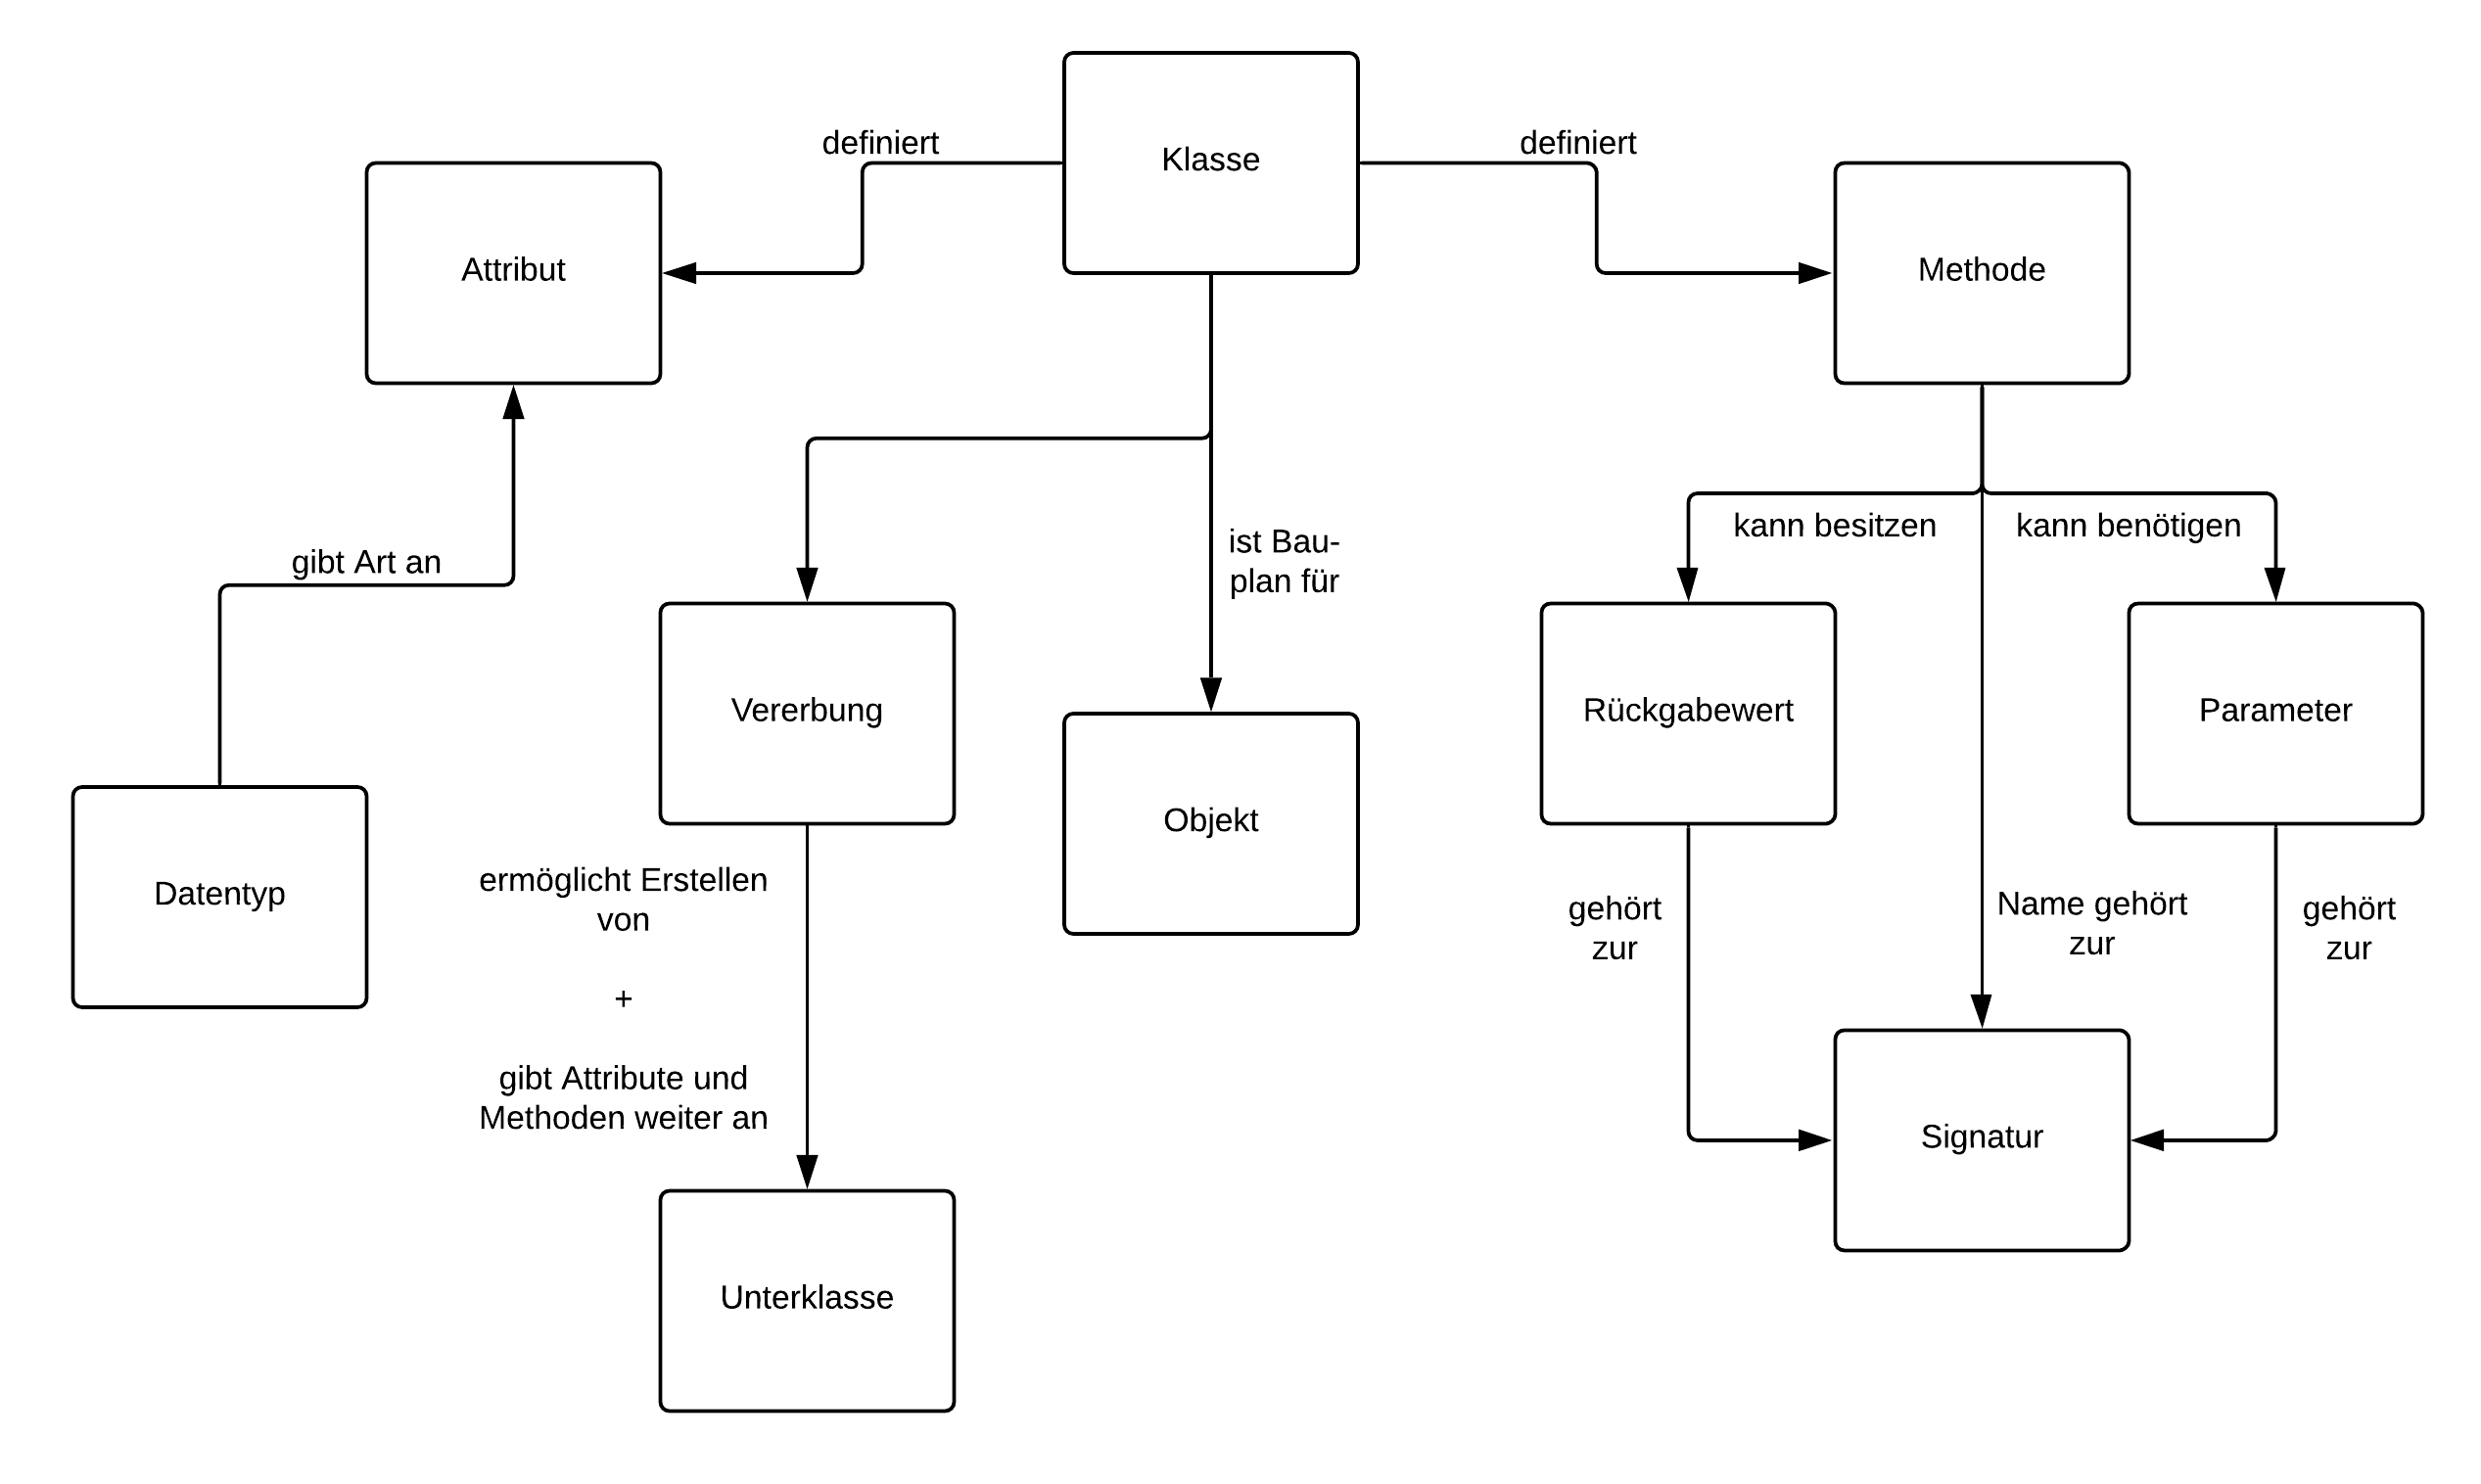
\includegraphics[height=7cm]{2.3.2.1/1.Basisversion/2-1.jpg}
\end{figure}

\newpage

\subsection{Fallunterscheidungen in Java}

\begin{figure}[ht]
	\centering
	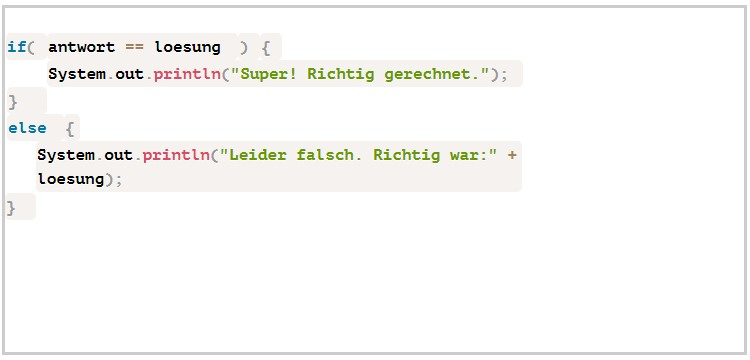
\includegraphics[height=7cm]{2.3.2.1/1.Basisversion/3-1.jpg}
\end{figure}

Auch hier ist es wichtig, die Syntax kennenzulernen.\\
Ein einfaches \glqq =\grqq{} bedeutet, dass der Variable links vom \glqq =\grqq{}-Zeichen der Wert auf der rechten Seite zugewiesen wird.\\
Ein zweifaches \glqq =\grqq{} bewirkt, dass überprüft wird, ob der Wert auf der linken Seite dem rechten entspricht.

\subsection{rateEinmal mit Rückgabe}

\begin{lstlisting}
boolean rateEinmal() {
    ...
    
    if (antwort == loesung) {
        System.out.println("Super! Richtig gerechnet.");
        return true;
    } else {
        System.out.println("Leider falsch. Richtig war:" + loesung);
        return false;
    }
}
\end{lstlisting}

\newpage

Damit die Methode zurückgeben kann, ob richtig oder falsch beantwortet wurde, ändert man den Rückgabetypen von \texttt{void} zu \texttt{boolean}.\\
Zuletzt gibt man \glqq wahr\grqq{} als Rückgabe an (\texttt{return true}), wenn die Antwort richtig war, bzw. \glqq falsch\grqq{}, falls die Antwort nicht richtig war (\texttt{return false}).

\subsection{eineRundeSpielen}

Ich gebe natürlich wieder die Lösung der Hilfe an, jedoch ist darunter eine (meiner Meinung nach) etwas einfachere und kürzere Version dieses Codes, Erklärungen folgen danach.\\

\begin{figure}[ht]
	\centering
	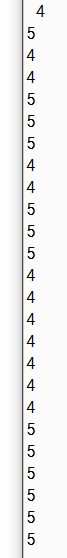
\includegraphics[height=12cm]{2.3.2.1/1.Basisversion/5-1.jpg}
\end{figure}

\newpage

\begin{lstlisting}
void eineRundeSpielen() {
    runden++;
    
    if (rateEinmal()) {
        punkte1++;
    }
    
    if (rateEinmal()) {
        punkte2++;
    }
    
    System.out.println("Spieler 1 hat " + punkte1 + "Punkt(e)");
    System.out.println("Spieler 2 hat " + punkte2 + "Punkt(e)");
    
    System.out.println(); //Fuer etwas Abstand zur naechsten Runde
}
\end{lstlisting}

Um eventuell Verwirrung vorzubeugen, hier eine Erklärung zu dem Ausdruck \texttt{if(rateEinmal())}:
Normalerweise erwartet man ein \texttt{==true} oder \texttt{==false}, wenn man diese Ausdrücke jedoch weglässt, wird automatisch von \texttt{==true} ausgegangen.\\
\texttt{if(rateEinmal())} bedeutet also soviel wie \texttt{if(rateEinmal() == true)}.

Nun zu meiner Variante:\\
Ich habe die Variablen \texttt{richtigGeraten} ausgelassen, da man direkt in der if-Bedingung die Methode aufrufen und so den boolean-Wert abfragen kann ohne extra dafür Variablen erstellen zu müssen.

Dadurch, dass ich zweimal eine if-Schleife mit der Methode \texttt{rateEinmal} als Bedingung aufgestellt habe, werden meist auch verschiedene Werte für die beiden Spieler erzeugt, da die Methode dementsprechend auch zweimal aufgerufen wird.\\
Außerdem habe ich in meiner Version die Addition von 1 wieder etwas vereinfacht (durch das \texttt{++}).

\newpage

\subsection{spielSteuern}

Die Schleife zum Erfüllen der Aufgabe, dass nämlich \texttt{eineRundeSpielen} aufgerufen werden soll, solange $\texttt{runden} < 5$ erfüllt ist, ist vorgegeben.

Der Rest ist mithilfe des angegebenen Struktogramms einfach umzusetzen, sodass ich nicht davon ausgehe, dass Fragen zu dem Code entstehen:\\
\begin{lstlisting}
void spielSteuern() {
    while (runden < 5) {
        eineRundeSpielen();
    }
    
    if (punkte1 == punkte2) {
        System.out.println("Unentschieden");
    } else {
        if (punkte1 > punkte2) {
            System.out.println("Spieler 1 hat gewonnen");
        } else {
            System.out.println("Spieler 2 hat gewonnen");
        }
    }
}
\end{lstlisting}

\subsection{Spielende}

Die grün markierten Ausdrücke sind geeignet, um die gewünschte Gewinnregel zu erfüllen:

\textcolor{darkred}{runden $< 10$ \&\& !(punkte1 $>= 5$ \&\& punkte2 $>= 5$)}\\
\textcolor{darkgreen}{(runden $< 10$ \&\& !(punkte1 $>= 5$)) \&\& (runden $< 10$ \&\& !(punkte2 $>= 5$))}\\
\textcolor{darkred}{(runden $< 10$ \&\& !(punkte1 $>= 5$)) $||$ (runden $< 10$ \&\& !(punkte2 $>= 5$))}\\
\textcolor{darkgreen}{runden $< 10$ \&\& !(punkte1 $>= 5$ $||$ punkte2 $>= 5$)}\\
\textcolor{darkgreen}{runden $< 10$ \&\& punkte1 $< 5$ \&\& punkte2 $< 5$}

\newpage

Einen der Ausdrücke setzt du jetzt nur noch in die while-Bedingung ein, dann kannst du es auch schon testen.

\subsection{Erste Anpassungen}

Ich nehme als Anpassungen, die ich machen möchte, die Beispiele, die aufgeführt wurden:

\begin{itemize}
    \barrow Ich möchte die Ausgabe insofern anpassen, dass statt \texttt{Spieler 1} bzw. \texttt{2} der Name benutzt wird, den man am Anfang angibt. Dies löse ich mithilfe des Konstruktors:\\
    \begin{lstlisting}
String spieler1;
String spieler2;
    
Spiel(String spieler1, String spieler2) {
    this.spieler1 = spieler1;
    this.spieler2 = spieler2;
}
    \end{lstlisting}
    
    Der Ausdruck \texttt{this.x = x} weist einer klassenweiten Variable, dem Attribut \texttt{x}, den Wert x aus der Methode (also in dem Fall den im Konstruktor anzugebenen Wert) zu.\\
    Zu beachten ist, dass die Namen im Konstruktor aufgrund des Datentypes in Anführungszeichen angegeben werden muss.
    
    Nun kann man in den Konsolenausgaben jeweils das \texttt{Spieler 1} bzw. \texttt{2} durch \texttt{spieler1} bzw. \texttt{2} ersetzen.
    \barrow Den Zahlenbereich kann man einfach durch Anpassen des Parameters ändern, mit welchem man die Methode \texttt{zufallszahl} aufruft, z.B. \texttt{zufallszahl(1000)}.
    \barrow Abschließend füge ich noch Zugriffsmodifikatoren bei Methoden und Attributen hinzu:
    
    \begin{lstlisting}
    private int runden;
    private int punkte1;
    private int punkte2;
    private String spieler1;
    private String spieler2;
    
    public Spiel(...) {
        ...
    }
    
    public void spielSteuern() {
        ...
    }
    
    private void eineRundeSpielen() {
        ...
    }
    
    private boolean rateEinmal() {
        ...
    }

    private int zufallszahl(...) {
        ...
    }

    private int leseZahl() {
        ...
    }
    \end{lstlisting}
    
    Das einzige, worauf der Nutzer zugreifen soll ist der Konstruktor und die Methode \texttt{spielSteuern}, da diese das Aufrufen der anderen Methoden übernimmt.
    
\end{itemize}

\newpage

\section{Fachkonzept - lokale Variablen}

Zu dieser Seite sind meines Erachtens nach keine Anleitungen und/oder Erläuterungen nötig.\\
Wenn doch Fragen aufkommen, schreib' einfach an \textbf{\href{mailto:nikodiamond3@gmail.com}{nikodiamond3@gmail.com}}.

\newpage

\section{Fachkonzept - Fallunterscheidung}

Zu dieser Seite sind meines Erachtens nach keine Anleitungen und/oder Erläuterungen nötig.\\
Wenn doch Fragen aufkommen, schreib' einfach an \textbf{\href{mailto:nikodiamond3@gmail.com}{nikodiamond3@gmail.com}}.

\newpage

\section{Fachkonzept - Bedingungen}

Zu dieser Seite sind meines Erachtens nach keine Anleitungen und/oder Erläuterungen nötig.\\
Wenn doch Fragen aufkommen, schreib' einfach an \textbf{\href{mailto:nikodiamond3@gmail.com}{nikodiamond3@gmail.com}}.

\newpage

\section{Übungen}

\subsection{Zufälliger Operator}

\begin{figure}[ht]
	\centering
	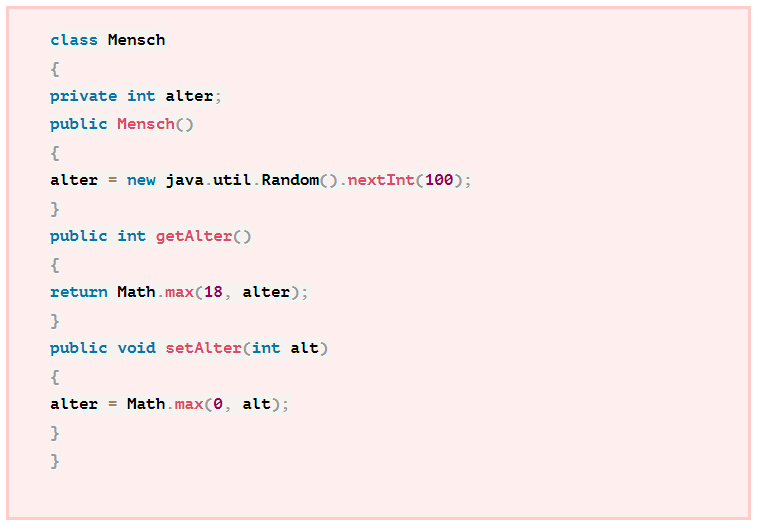
\includegraphics[height=18cm]{2.3.2.1/5.Uebungen/1-1.png}
\end{figure}

\newpage

\subsection{Zeitmessung}

Bei dieser Aufgabe muss ziemlich viel angepasst werden, um die Zeitmessung zu implementieren.

Da die while-Bedingung nun nicht mehr die Runden und die Punktzahl beinhaltet, soll sie jetzt aus Punktzahl und der Restzeit pro Spieler bestehen. Daher kann das Runden-Attribut nun entfernt werden. Stattdessen habe ich für beide Spieler analog zu der Punktzahl ein Restzeit-Attribut hinzugefügt, diese habe ich dann in die while-Bedingung eingebaut.

Die Zeit, die man nun also benötigt, um eine Aufgabe zu lösen, wird in einem Attribut gespeichert und später von der Restzeit des Spielers abgezogen. Zusätzlich dazu wird die verbrauchte und die verbleibende Zeit ausgegeben.\\

Da der Code dazu nun  stark angepasst wurde, hier mein Quellcode:\\
\begin{lstlisting}
class Spiel {
    private int punkte1;
    private int punkte2;
    private String spieler1;
    private String spieler2;
    private int restzeit1;
    private int restzeit2;
    private int gebrauchteZeit;
    
    public Spiel(String spieler1, String spieler2) {
        restzeit1 = 30;
        restzeit2 = 30;
        this.spieler1 = spieler1;
        this.spieler2 = spieler2;
    }
    
    public void spielSteuern() {
        while (punkte1 < 5 && punkte2 < 5 && restzeit1 > 0 && restzeit2 > 0) {
            eineRundeSpielen();
        }
        
        if (punkte1 == punkte2) {
            System.out.println("Unentschieden");
        } else {
            if (punkte1 > punkte2) {
                System.out.println(spieler1 + " hat gewonnen");
            } else {
                System.out.println(spieler2 + " hat gewonnen");
            }
        }
    }
    
    private void eineRundeSpielen() {        
        if (rateEinmal()) {
            punkte1++;
            restzeit1 -= gebrauchteZeit;
            System.out.println("Restzeit: " + restzeit1 + " Sekunden");
        } else {
            restzeit1 -= gebrauchteZeit;
            System.out.println("Restzeit: " + restzeit1 + " Sekunden");
        }
        
        if (rateEinmal()) {
            punkte2++;
            restzeit2 -= gebrauchteZeit;
            System.out.println("Restzeit: " + restzeit2 + " Sekunden");
        } else {
            restzeit2 -= gebrauchteZeit;
            System.out.println("Restzeit: " + restzeit2 + " Sekunden");
        }
        
        System.out.println(spieler1 + " hat " + punkte1 + "Punkt(e).");
        System.out.println(spieler2 + " hat " + punkte2 + "Punkt(e).");
        
        System.out.println();
    }
    
    private boolean rateEinmal() {
        int zahl1;
        int zahl2;
        int loesung;
        String operator;
        int operatorNummer = zufallszahl(4);
        
        if (operatorNummer == 0) {
            operator = "+";
            zahl1 = zufallszahl(100) + 100;
            zahl2 = zufallszahl(100) + 100;
            loesung = zahl1 + zahl2;
        } else if (operatorNummer == 1) {
            operator = "-";
            zahl1 = zufallszahl(100) + 100;
            zahl2 = zufallszahl(100) + 100;
            loesung = zahl1 - zahl2;
        } else if (operatorNummer == 2) {
            operator = "*";
            zahl1 = zufallszahl(15) + 1;
            zahl2 = zufallszahl(15) + 1;
            loesung = zahl1 * zahl2;
        } else {
            operator = "/";
            loesung = zufallszahl(10);
            zahl2 = zufallszahl(9) + 1;
            zahl1 = zahl2 * loesung;
        }
        
        System.out.println("Wie viel ist " + zahl1 + operator + zahl2 + "?");
        int start = (int)(System.currentTimeMillis() / 1000);
        int antwort = leseZahl();
        int ende = (int)(System.currentTimeMillis() / 1000);
        gebrauchteZeit = ende - start;
        
        if (antwort == loesung) {
            System.out.println("Super! Richtig gerechnet.");
            System.out.println("Du hast " + gebrauchteZeit + " Sekunden gebraucht.");
            return true;
        } else {
            System.out.println("Leider falsch. Richtig war:" + loesung);
            System.out.println("Du hast " + gebrauchteZeit + " Sekunden gebraucht.");
            return false;
        }
    }

    private int zufallszahl(int n) {
        return new java.util.Random().nextInt(n);
    }

    private int leseZahl() {
        return new java.util.Scanner(System.in).nextInt();
    }
}
\end{lstlisting}

\subsection{Eigene Erweiterungen}

Hier ist wieder deine Kreativität gefragt, viel Spaß beim Implementieren deiner Ideen.\\
Bei Fragen, einfach an \textbf{\href{mailto:nikodiamond3@gmail.com}{nikodiamond3@gmail.com}} schreiben.

\subsection{Fehlermeldung}

\begin{itemize}
    \barrow Die erste Fehlermeldung erscheint, da nach dem Zurückgeben eines boolean-Wertes die Methode beendet wird und die letzte Zeile in diesem Beispiel gar nicht erst aufgerufen werden kann.
    
    \newpage
    
    \barrow Hier entsteht eine Fehlermeldung, da in der letzten Zeile versucht wird, den String \texttt{s} auszugeben, jedoch ist \texttt{s} nur innerhalb der beiden Klammern definiert. Außerhalb der Klammern kann nicht mehr darauf zugegriffen werden.
\end{itemize}

\subsection{Typische Fehler}

\begin{itemize}
    \barrow \textbf{Fehler 1:}\\
    Wenn es zwei Variablen desselben Namens gibt, wird bei Benutzung die lokale Variable bevorzugt. Auf das Attribut kann mit \texttt{this.variable} zugegriffen werden.\\
    Somit wird hier der lokalen Variable \texttt{runden} der Wert derselben Variable zugewiesen, das klassenweite Attribut \texttt{runden} wird nicht verändert.
    \barrow \textbf{Fehler 2:}\\
    Die Zuweisung ist falsch herum aufgestellt. Mit dem Beispielcode wird der lokalen Variable \texttt{ r} der Wert von \texttt{runden} zugewiesen, bevor sie entfernt wird.\\
    Es müsste dem Attribut \texttt{runden} der Wert von \texttt{r} zugewiesen werden, ansonsten ändert sich \texttt{runden} auch hier nicht.
    \barrow \textbf{Fehler 3:}\\
    Bei der Zuweisung müsste man das \texttt{int} weglassen, da die Variable \texttt{runden} im Konstruktor nicht neu implementiert werden darf, da sonst die Variable wieder nur lokal existiert und nach Konstruktor-Aufruf wieder entfernt wird. Auch hier würde sich die klassenweite \texttt{runden}-Variable nicht ändern.
\end{itemize}

\subsection{Lokal vs. Attribut}

Beispiel 1 funktioniert, da bei Implementierung eines Attributs als Integer automatisch der Wert 0 zugewiesen wird.\\
Im Beispiel 2 funktioniert es nicht, da bei Implementierung einer lokalen Variable keine automatische Zuweisung erfolgt und sie gar keinen Wert besitzt.

\newpage

\subsection{Logische Ausdrücke}

\begin{figure}[ht]
	\centering
	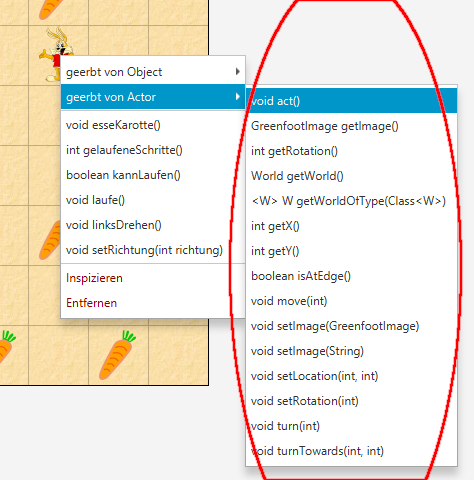
\includegraphics[height=9cm]{2.3.2.1/5.Uebungen/7-1.png}
\end{figure}

\subsection{Maximum-Funktion}

\begin{itemize}
    \barrow \textbf{max1:}\\
    Diese Methode funktioniert wie erwartet. Wenn \texttt{a} größer ist als \texttt{b}, wird \texttt{a} zurückgegeben, ansonsten (also sowohl wenn \texttt{b} größer ist als auch wenn \texttt{b} gleich groß ist wie \texttt{a}) wird \textbf{b} zurückgegeben (weil wenn sie gleich groß sind, ist es egal, ob \texttt{a} oder \texttt{b} zurückgegeben wird).
    \barrow \textbf{max2:}\\
    Diese Methode funktioniert auch wie erwartet, denn sie gleicht der ersten Methode stark. Es wurde einfach das \texttt{else} weggelassen, denn wenn die if-Bedingung erfüllt ist, wird \texttt{a} zurückgegeben und die Methode beendet, sodass die letzte Zeile nicht mehr durchgeführt wird.
    
    \newpage
    
    \barrow \textbf{max3:}\\
    Diese Methode funktioniert nicht aufgrund von einem fehlenden return-Statements. Wenn keine der beiden if-Bedingungen erfüllt ist (was in diesem Beispiel nicht funktionieren kann, aber generell zu beachten ist), gibt es kein return-Statement, welches man ausführen kann.\\
    Ich sehe nur eine Lösungsmöglichkeit, wenn man die beiden Bedingungen beibehalten möchte:
    
    \texttt{return 0} am Ende einfügen
\end{itemize}

\subsection{Bruch-Klasse}

Ob eine Zahl durch eine andere teilbar ist, lässt sich mit dem modulo-Operator überprüfen. Der Modulo gibt den Rest einer Division an.

10 mod 3 (sprich \glqq zehn Modulo drei\grqq{})\footnote{Modulo (mod) berechnen, mathe24, http://www.mathe24.net/modulo.html, (Abgerufen: 11.02.20, 17:58)} z.B. ergibt also 1.

Um also zu testen, ob der Zähler bzw. Nenner durch \texttt{k} teilbar ist, geben wir in der Methode \texttt{kuerzbarMit} true zurück, falls der Modulo 0 ist.

\begin{lstlisting}
boolean kuerzbarMit(int k) {
    if ((zaehler % k == 0) && (nenner % k == 0)) {
        return true;
    } else {
        return false;
    }
}
\end{lstlisting}

\newpage

Um diese Methode nun benutzen zu können, baut man diese dann in die Methode \texttt{kuerzen} ein.

\begin{lstlisting}
void kuerzen(int k) {
    if (kuerzbarMit(k)) {
        zaehler = zaehler / k;
        nenner = nenner / k;
    }
}
\end{lstlisting}

\end{document}